%%%%%%%%%%%%%%%%%%%%%%%%%%%%%%%%%%%%%%%%%%%%%%%%%%%%%%%%%%%%%%%%%%%%%%
%%                       IAEW LaTeX Template                        %%
%%%%%%%%%%%%%%%%%%%%%%%%%%%%%%%%%%%%%%%%%%%%%%%%%%%%%%%%%%%%%%%%%%%%%%
% ANGELEGT am 15.09.2026, Entscheidung V6 (A2). Traegt die Herleitung der
% zulaessigen Ueberlastdauer, die bis dahin in Abschnitt 2.1.2 stand, mit den
% Befunden B66, B67 und B68 des Betreuers. Die alte Fassung steht als
% Kommentar in chapters/chapter_2.tex.
\chapter{Zulässige Überlastdauer von Freileitung und Transformator}
\label{anh:thermik}

Dieser Anhang trägt die Herleitung der zulässigen Überlastdauer, auf die Abschnitt~\ref{sec:curative_functionality} verweist.
Die Wärmebilanz einer Freileitung lautet in der für eine Überlast maßgeblichen transienten Form nach \cite{cigre_thermal_2014}
\begin{equation}
    m\,c_{\mathrm{p}}\,\frac{\mathrm{d}\vartheta}{\mathrm{d}t} = P_{\mathrm{J}}(I,\vartheta) + P_{\mathrm{S}} - P_{\mathrm{C}}(\vartheta,\vartheta_{\mathrm{u}},v_{\mathrm{w}},\delta) - P_{\mathrm{R}}(\vartheta,\vartheta_{\mathrm{u}})
    \label{eq:waermebilanz}
\end{equation}
mit der mittleren Leitertemperatur $\vartheta$, der Wärmekapazität $m\,c_{\mathrm{p}}$, der ohmschen Verlustwärme $P_{\mathrm{J}}$, dem solaren Eintrag $P_{\mathrm{S}}$, der konvektiven und der Strahlungskühlung $P_{\mathrm{C}}$ und $P_{\mathrm{R}}$ sowie dem Anströmwinkel des Windes $\delta$.
Magnetische Erwärmung und Verdunstungskühlung sind nicht aufgeführt, und die Wärmekapazität ist als konstant angesetzt, sodass Gleichung~\ref{eq:waermebilanz} einen blanken Leiter im Freien beschreibt.

Die Kühlung hängt von den Wetterbedingungen ab und wächst unterproportional mit der Windgeschwindigkeit, weshalb windschwache Stunden die kürzeste zulässige Dauer ergeben \cite{cigre_thermal_2014}.
Das Freileitungsmonitoring erschließt dieses witterungsabhängige Potenzial bereits, indem es den dauerhaft zulässigen Grenzwert an die vorliegenden Bedingungen anpasst \cite{dena_hoeherauslastung_2022}.
Die kurative Höherauslastung setzt demgegenüber auf der Erwärmungsseite an, denn die ohmsche Verlustwärme wächst bei gegebener Leitertemperatur quadratisch mit dem Strom und lautet
\begin{equation}
    P_{\mathrm{J}}(I,\vartheta) = I^{2}\,R'_{20}\left[1 + \alpha_{20}\left(\vartheta - \vartheta_{20}\right)\right]
    \label{eq:jouleverluste}
\end{equation}
mit dem längenbezogenen Widerstand $R'_{20}$ bei der Bezugstemperatur $\vartheta_{20}$ und dem Temperaturkoeffizienten $\alpha_{20}$.
Vernachlässigt sind dabei der Skineffekt, also die Verdrängung des Stroms an den äußeren Rand des Leiterseils, die den wirksamen Widerstand bei Wechselstrom erhöht, sowie die Nichtlinearität des Widerstands bei hohen Temperaturen.
Eine Erhöhung des Stroms um zehn Prozent steigert den Wärmeeintrag nach Gleichung~\ref{eq:jouleverluste} damit um rund ein Fünftel.
Genutzt wird nicht die stationäre Kühlung, sondern die Wärmekapazität des Betriebsmittels, die einen Strom oberhalb des Dauergrenzwerts für eine begrenzte Zeit zulässt.
Bei einer Überlast überwiegt der Wärmeeintrag, und die Leitertemperatur steigt vom Ausgangswert, der aus der Vorbelastung folgt, derjenigen Temperatur zu, bei der sich Wärmeeintrag und Kühlung wieder ausgleichen.
Die Überlast ist zulässig, bis die Grenztemperatur erreicht ist, denn oberhalb der Grenztemperatur nehmen Durchhang und Festigkeit des Leiterseils unzulässige Werte an, und aus dieser Dauer folgt die der jeweiligen Überlasthöhe zugeordnete zulässige Dauer.
Abbildung~\ref{fig:tatl_berechnung} zeigt die Eingangsgrößen und den daraus folgenden Temperaturverlauf.

\begin{figure}[htbp]
    \centering
% GROESSENANGABE ERGAENZT am 12.09.2026 nach der Anweisung des Verfassers.
% Sie aendert den Satz nicht, die Datei ist genau textbreit.
    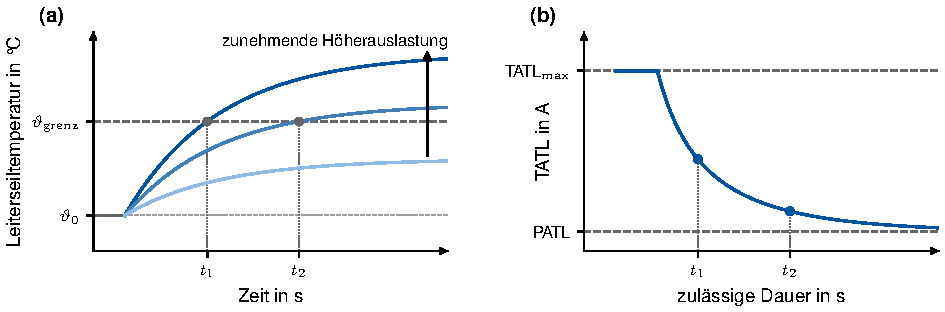
\includegraphics[width=\textwidth]{figures/chapter_2/tatl_berechnung.pdf}
    \caption{Schematische Darstellung der zulässigen Überlastdauer einer Freileitung. Teilbild a zeigt die Temperaturverläufe für drei Überlasthöhen, Teilbild b die daraus folgende Kennlinie aus zulässiger Belastbarkeit und zulässiger Dauer.}
    \label{fig:tatl_berechnung}
\end{figure}

Für Transformatoren gilt derselbe Mechanismus mit drei Unterschieden.
Maßgebliche Größe ist dort die Heißpunkttemperatur der Wicklung, die über die Öltemperatur und den Ölumlauf mit der Umgebung verbunden ist, sodass zwischen der Verlustentstehung in der Wicklung und der Wärmeabgabe an die Umgebungsluft ein zusätzlicher innerer Transportweg liegt.
Die Wärmekapazität eines Transformators ist größer, weshalb die zulässigen Überlastdauern länger ausfallen als bei einer Freileitung.
Die Temperatur steht bei beiden Betriebsmitteln für eine Wirkung, nämlich für Durchhang und Festigkeit am Leiterseil und für die Alterung der Isolation am Transformator, und beim Transformator summiert sich diese Wirkung über die Einsätze, weil jede Überlast einen Anteil der Lebensdauer verbraucht, sodass neben Höhe und Dauer auch die Häufigkeit der Überlastung zu begrenzen ist \cite{iec_60076_7_2018}.
